%%%%%%%%%%%%%%%%%%%%%%%%%%%%%%%%%%%%%%%%%%%%%%%%%%%%%%%%%%%%%%%%%%%%%%
%%%%%%%%%%%%%%%%%%%%%%%%%%%%%%%%%%%%%%%%%%%%%%%%%%%%%%%%%%%%%%%%%%%%%%
%%%%%%%%%%%%%%%%%%%%%%%%%%%%%%%%%%%%%%%%%%%%%%%%%%%%%%%%%%%%%%%%%%%%%%
%%%%%%%%%%%%%%%%%%%%%%%%%%%%%%%%%%%%%%%%%%%%%%%%%%%%%%%%%%%%%%%%%%%%%%
\chapter{Asservissements linéaires des systèmes\label{chap-asservis}}
%%%%%%%%%%%%%%%%%%%%%%%%%%%%%%%%%%%%%%%%%%%%%%%%%%%%%%%%%%%%%%%%%%%%%%
%%%%%%%%%%%%%%%%%%%%%%%%%%%%%%%%%%%%%%%%%%%%%%%%%%%%%%%%%%%%%%%%%%%%%%
%%%%%%%%%%%%%%%%%%%%%%%%%%%%%%%%%%%%%%%%%%%%%%%%%%%%%%%%%%%%%%%%%%%%%%
%%%%%%%%%%%%%%%%%%%%%%%%%%%%%%%%%%%%%%%%%%%%%%%%%%%%%%%%%%%%%%%%%%%%%%

%%%%%%%%%%%%%%%%%%%%%%%%%%%%%%%%%%%%%%%%%%%%%%%%%%%%%%%%%%%%%%%%%%%%%%
%%%%%%%%%%%%%%%%%%%%%%%%%%%%%%%%%%%%%%%%%%%%%%%%%%%%%%%%%%%%%%%%%%%%%%
%%%%%%%%%%%%%%%%%%%%%%%%%%%%%%%%%%%%%%%%%%%%%%%%%%%%%%%%%%%%%%%%%%%%%%
\section{Introduction}
%%%%%%%%%%%%%%%%%%%%%%%%%%%%%%%%%%%%%%%%%%%%%%%%%%%%%%%%%%%%%%%%%%%%%%
%%%%%%%%%%%%%%%%%%%%%%%%%%%%%%%%%%%%%%%%%%%%%%%%%%%%%%%%%%%%%%%%%%%%%%
%%%%%%%%%%%%%%%%%%%%%%%%%%%%%%%%%%%%%%%%%%%%%%%%%%%%%%%%%%%%%%%%%%%%%%


\begin{figure}[!h]
    \centering
        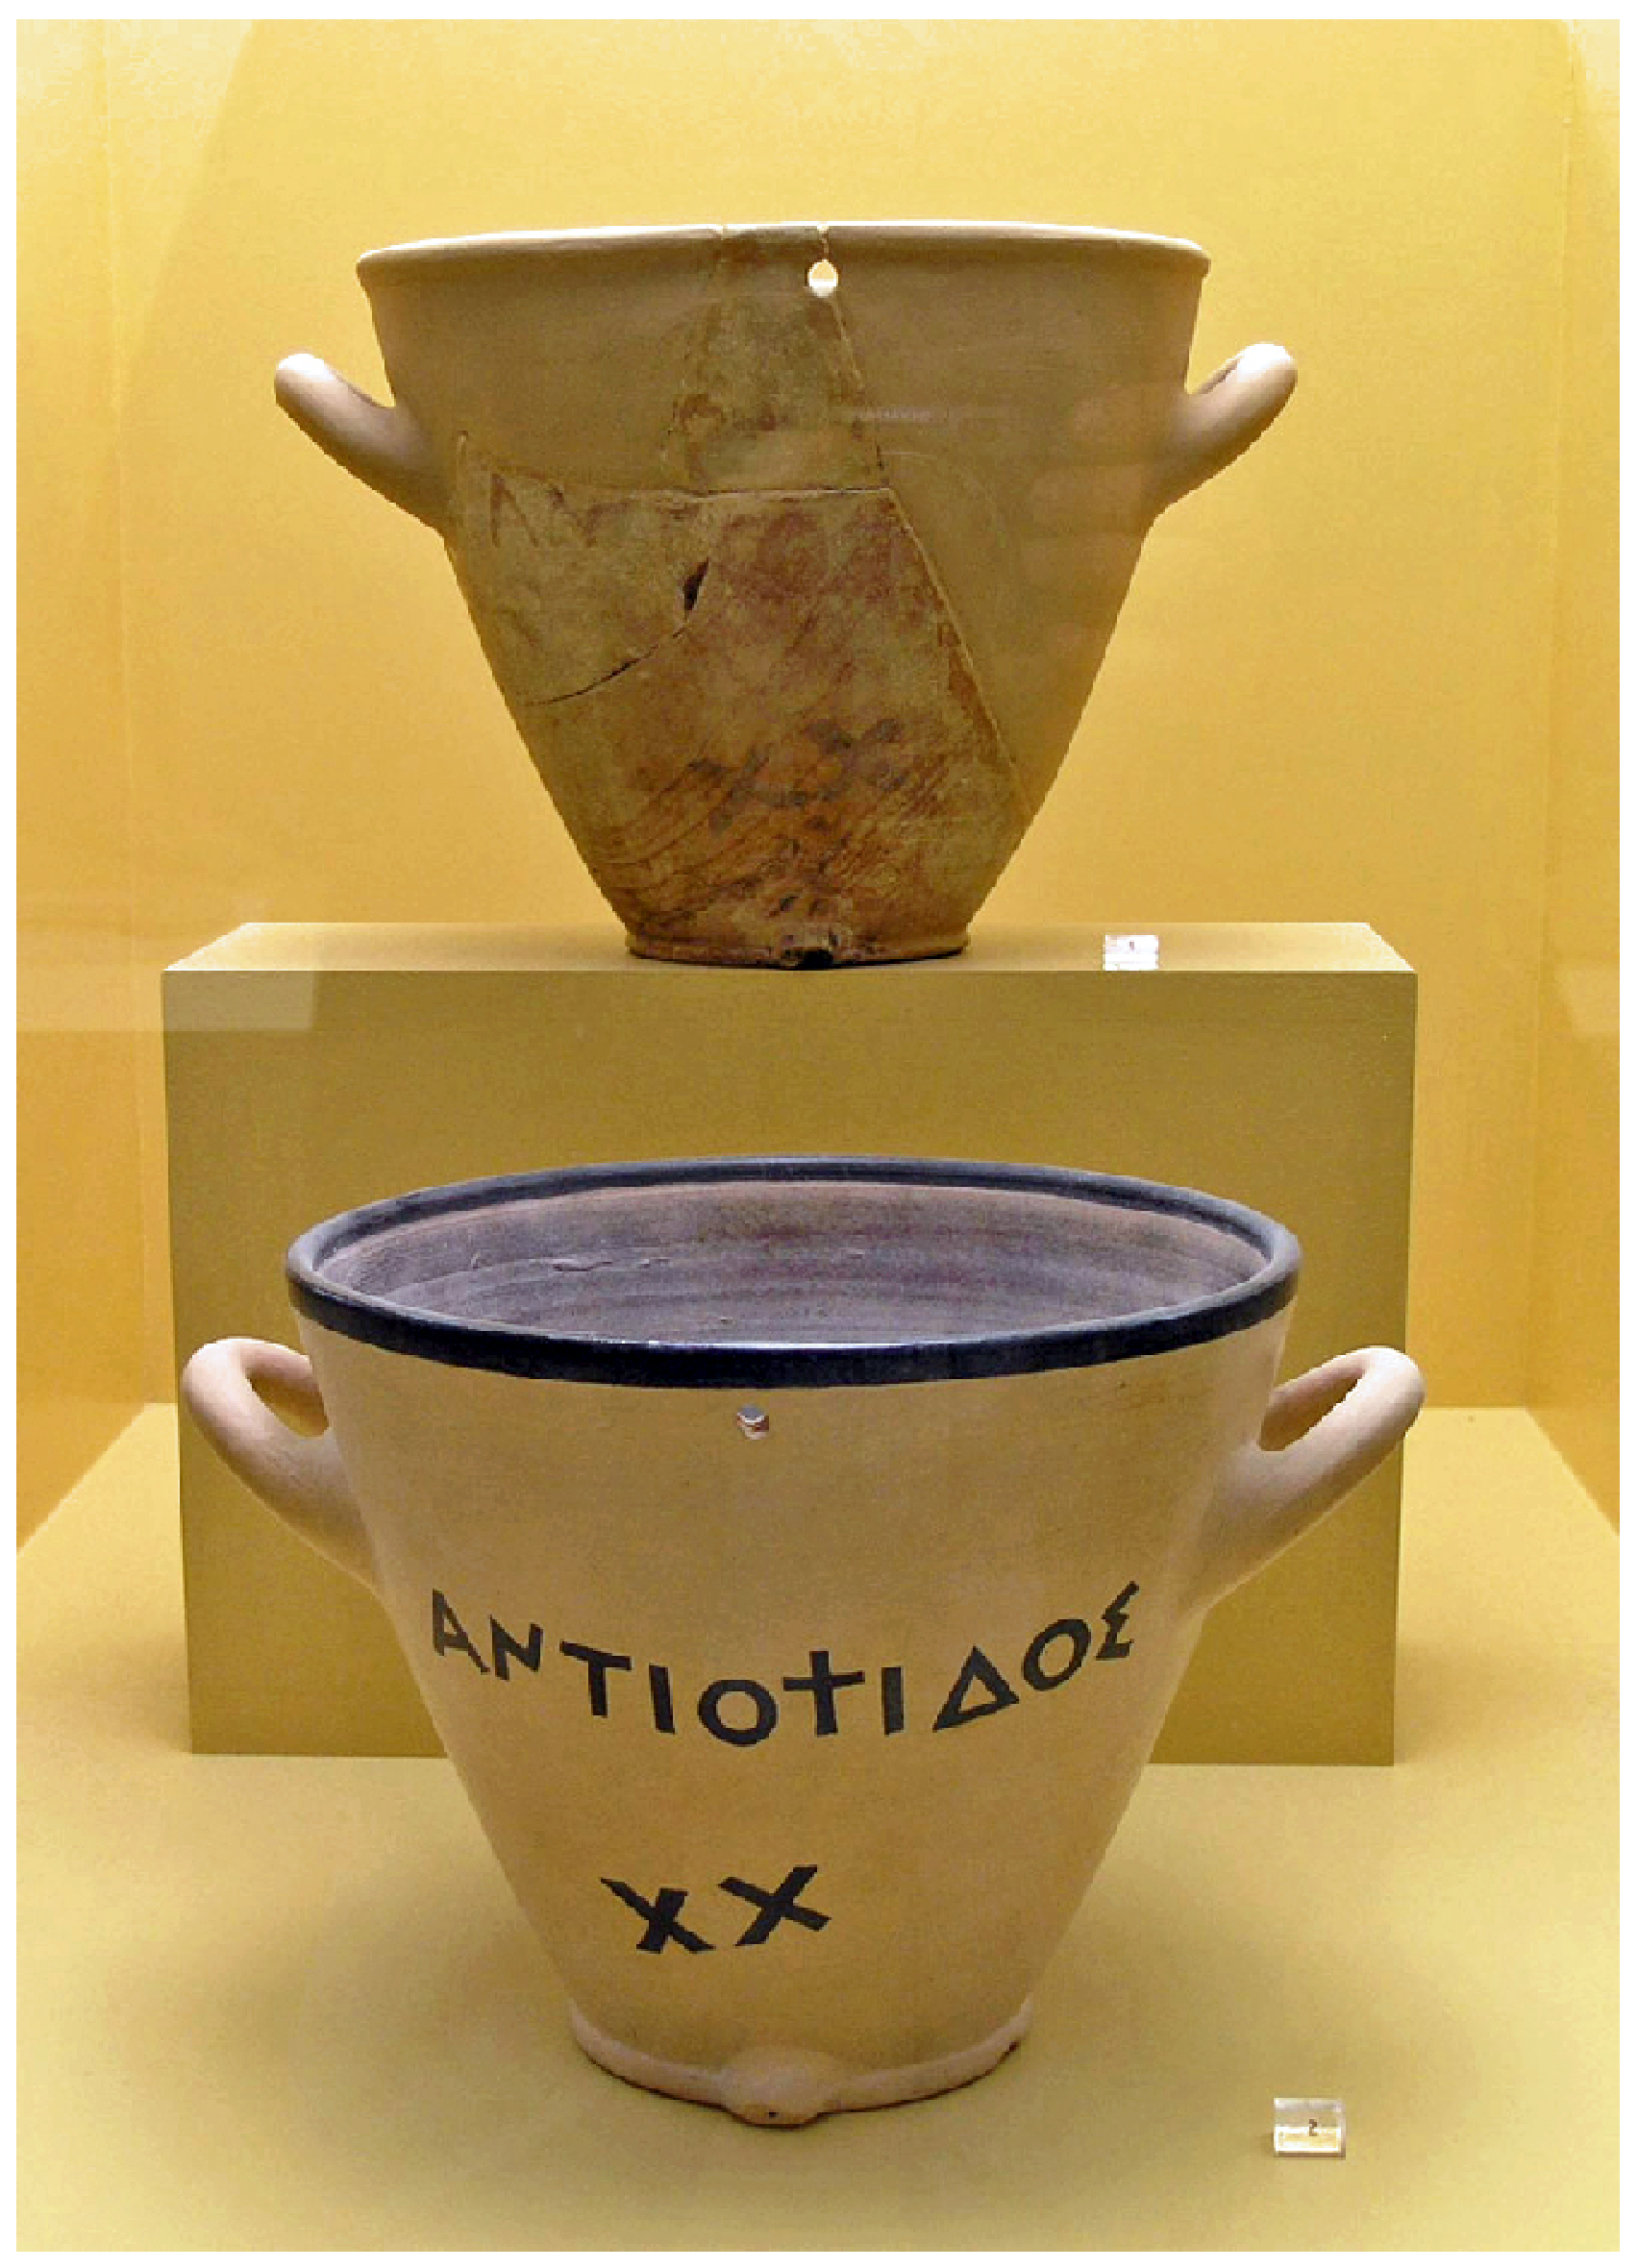
\includegraphics[width=0.45\linewidth,height=10cm]{fig/AGMA_Clepsydre_m.eps}
        \label{fig-clep}
        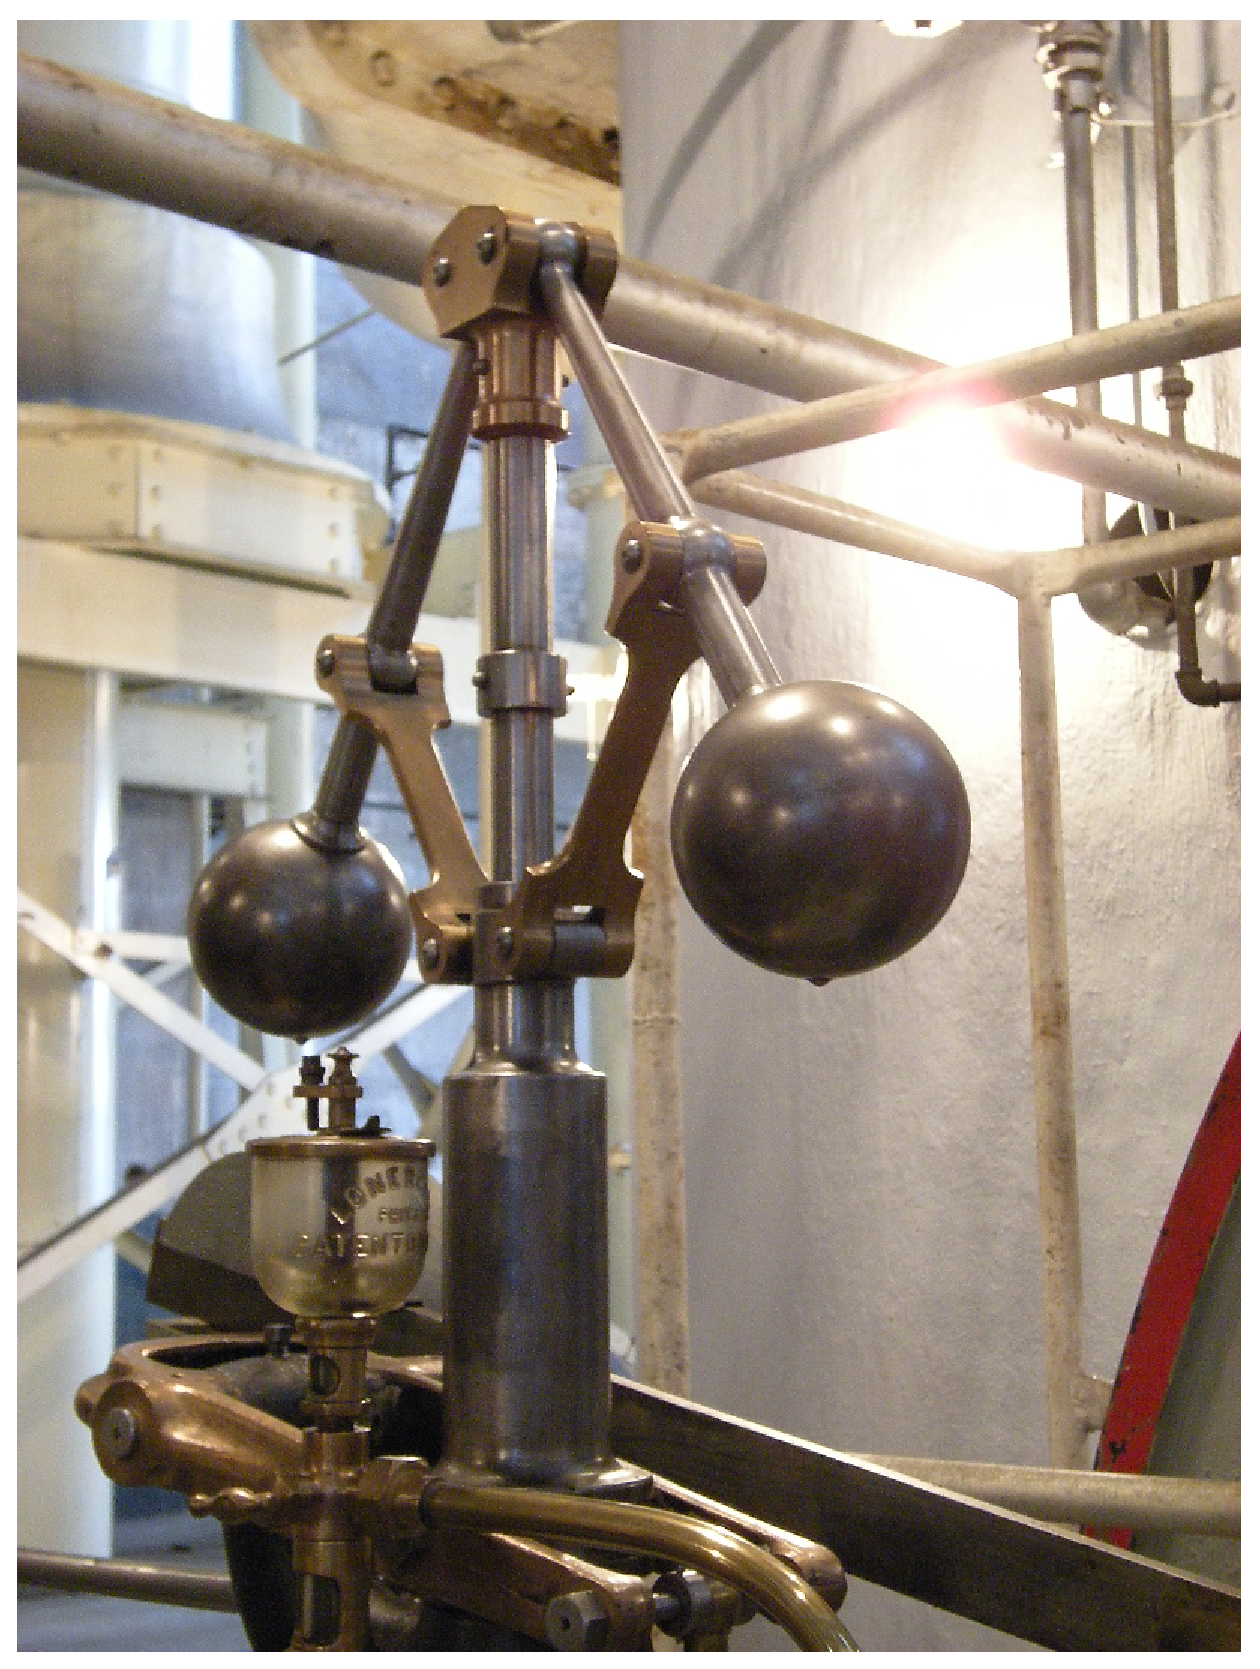
\includegraphics[width=0.45\linewidth,height=10cm]{fig/Georgetown_PowerPlant_Museum_m.eps}
        \label{fig-watt}
    \caption{Exemples historiques de régulateurs.\label{fig-hist}}
\end{figure}

%%%%%%%%%%%%%%%%%%%%%%%%%%%%%%%%%%%%%%%%%%%%%%%%%%%%%%%%%%%%%%%%%%%%%%
%%%%%%%%%%%%%%%%%%%%%%%%%%%%%%%%%%%%%%%%%%%%%%%%%%%%%%%%%%%%%%%%%%%%%%
%%%%%%%%%%%%%%%%%%%%%%%%%%%%%%%%%%%%%%%%%%%%%%%%%%%%%%%%%%%%%%%%%%%%%%
\section{Organisation d'un asservissement}
%%%%%%%%%%%%%%%%%%%%%%%%%%%%%%%%%%%%%%%%%%%%%%%%%%%%%%%%%%%%%%%%%%%%%%
%%%%%%%%%%%%%%%%%%%%%%%%%%%%%%%%%%%%%%%%%%%%%%%%%%%%%%%%%%%%%%%%%%%%%%
%%%%%%%%%%%%%%%%%%%%%%%%%%%%%%%%%%%%%%%%%%%%%%%%%%%%%%%%%%%%%%%%%%%%%%

%%%%%%%%%%%%%%%%%%%%%%%%%%%%%%%%%%%%%%%%%%%%%%%%%%%%%%%%%%%%%%%%%%%%%%
%   Nom des noeuds
%                                      
%   E ---- a ---- b ---- c ---- S
%          |                |
%          |                |
%            ---- d ------- 
% E : entrée
% a : comparateur
% b : correcteur
% c : système
% S : sortie
% d : capteur
% r : noeud décalé pour le retour
%%%%%%%%%%%%%%%%%%%%%%%%%%%%%%%%%%%%%%%%%%%%%%%%%%%%%%%%%%%%%%%%%%%%%%
\begin{center}
    \begin{tikzpicture}
        \sbEntree{E}
        \sbComp{a}{E}
        \sbRelier[$E(p)$]{E}{a}           % entree
        \sbBloc[3]{b}{$C(p)$}{a}
        \sbRelier[$\epsilon(p)$]{a}{b}    % ecart
        \sbBloc[3]{c}{$H(p)$}{b}
        \sbRelier[$U(p)$]{b}{c}           % commande
        \sbSortie[4]{S}{c}
        \sbRelier{c}{S}
        \sbNomLien[0.8]{S}{$S(p)$}
        \sbDecaleNoeudy[6]{b-c}{r}
        \sbBlocr[-1.6]{d}{$G(p)$}{r}
        \sbRelieryx{c-S}{d}              
        \sbRelierxy[$M(p)$]{d}{a}         % mesure (image de S)
        \node[yshift=-0.8em] at (b.south) {\small Correcteur};
        \node[yshift=-0.8em] at (c.south) {\small Système};
        \node[yshift=-0.8em] at (d.south) {\small Capteur};
        \node[yshift=-0.8em,xshift=0.5em] at (E.south) {\small Consigne};
        \node[yshift=-0.8em] at (S.south) {\small Sortie};
    \end{tikzpicture}
\end{center}

\begin{center}
    \begin{tikzpicture}
        \sbEntree{E}
        \sbComp{a}{E}
        \sbRelier[$E(p)$]{E}{a}           % entree
        \sbBloc[3]{b}{$C(p)$}{a}
        \sbRelier[$\epsilon(p)$]{a}{b}    % ecart
        \sbBloc[4.2]{c}{$H(p)$}{b}
        \sbRelier[$U(p)$]{b}{c}           % commande
        \sbSortie[4]{S}{c}
        \sbRelier{c}{S}
        \sbNomLien[0.8]{S}{$S(p)$}
        \sbDecaleNoeudy[7]{b-c}{r}
        \sbBlocr[-1.6]{d}{$G(p)$}{r}
        \sbRelieryx{c-S}{d}              
        \sbRelierxy[$M(p)$]{d}{a}         % mesure (image de S)
        \node[yshift=-0.8em] at (b.south) {\small Correcteur};
        \node[yshift=-0.8em] at (c.south) {\small Système};
        \node[yshift=-0.8em] at (d.south) {\small Capteur};
        \draw[dashed,very thick,blue] (1.15,-1.8) rectangle node[blue,xshift=-1.999999999em,yshift=4em] {\textbf{Régulateur}} (4.9,1);
    \end{tikzpicture}
\end{center}

%%%%%%%%%%%%%%%%%%%%%%%%%%%%%%%%%%%%%%%%%%%%%%%%%%%%%%%%%%%%%%%%%%%%%%
%   Nom des noeuds
%                                      
%                                      
%   E ---- a ---- b ---- c ---- d ---- e ---- S
%                 |                       |
%                 |                       |
%                  --------- f -----------
% E : entrée
% a : adaptateur 
% b : comparateur
% c : correcteur
% d : actionneur
% e : système
% S : sortie
% f : capteur
% r : noeud décalé pour le retour
%%%%%%%%%%%%%%%%%%%%%%%%%%%%%%%%%%%%%%%%%%%%%%%%%%%%%%%%%%%%%%%%%%%%%%
\begin{center}
    \begin{tikzpicture}
        \sbEntree{E}
        \sbBloc[3]{a}{$A_d(p)$}{E}
        \sbRelier[$E(p)$]{E}{a}
        \sbComp{b}{a}
        \sbRelier{a}{b}
        \sbBloc[3]{c}{$C(p)$}{b}
        \sbRelier[$\epsilon(p)$]{b}{c}
        \sbBloc[3]{d}{$A_c(p)$}{c}
        \sbRelier[$\epsilon'(p)$]{c}{d}
        \sbBloc[3]{e}{$H(p)$}{d}
        \sbRelier[$U(p)$]{d}{e}
        \sbSortie[4]{S}{e}
        \sbRelier{e}{S}
        \sbDecaleNoeudy[5]{d}{r}
        \sbBlocr[-1.6]{f}{$G(p)$}{r}
        \sbRelieryx{e-S}{f}              
        \sbRelierxy[$M(p)$]{f}{b}        % Mesure
        \sbNomLien[0.8]{S}{$S(p)$}
    \end{tikzpicture}
\end{center}

%%%%%%%%%%%%%%%%%%%%%%%%%%%%%%%%%%%%%%%%%%%%%%%%%%%%%%%%%%%%%%%%%%%%%%
%   Nom des noeuds
%                                      P
%                                      |
%                                      |
%   E ---- a ---- b ---- c ---- d ---- e ---- f ---- S
%                 |                              |
%                 |                              |
%                  ------------ g ---------------
% E : entrée
% a : adaptateur 
% b : comparateur
% c : correcteur
% d : actionneur
% e : sommateur (perturbation)
% P : perturbation
% f : système 
% S : sortie
% g : capteur
% r : noeud décalé pour le retour
%%%%%%%%%%%%%%%%%%%%%%%%%%%%%%%%%%%%%%%%%%%%%%%%%%%%%%%%%%%%%%%%%%%%%%
\begin{landscape}
\vspace*{\fill}
\begin{center}
    \begin{tikzpicture}
        \sbEntree{E}
        \sbBloc[3]{a}{$A_d(p)$}{E}
        \sbRelier[$E(p)$]{E}{a}
        \sbComp{b}{a}
        \sbRelier{a}{b}
        \sbBloc[3]{c}{$C(p)$}{b}
        \sbRelier[$\epsilon(p)$]{b}{c}
        \sbBloc[3]{d}{$A_c(p)$}{c}
%        \sbRelier[$\epsilon'(p)$]{c}{d}
        \sbRelier{c}{d}
        \sbSumh[6.7]{e}{d}
        \sbDecaleNoeudy[-3]{e}{P}
        \sbRenvoiF[-3]{P}{e}{$P(p)$}
        \sbRelier[$U(p)$]{d}{e}
        \sbBloc{f}{$H(p)$}{e}
        \sbRelier{e}{f}
        \sbSortie[4]{S}{f}
        \sbRelier{f}{S}
        \sbDecaleNoeudy[5]{c}{r}
        \sbBlocr[-1.6]{g}{$G(p)$}{r}
        \sbRelieryx{f-S}{g}              
        \sbRelierxy[$M(p)$]{g}{b}        
        \sbNomLien[0.8]{S}{$S(p)$}
        \node[yshift=-0.8em] at (a.south) {\small Adaptateur};
        \node[yshift=-0.8em] at (c.south) {\small Correcteur};
        \node[yshift=-0.8em] at (d.south) {\small Actionneur};
        \node[yshift=-0.8em] at (f.south) {\small Système};
        \node[yshift=-0.8em] at (g.south) {\small Capteur};
        \node[yshift=-0.8em,xshift=0.5em] at (E.south) {\small Consigne};
        \node[yshift=-0.8em] at (S.south) {\small Sortie};
        \node[yshift=2em,xshift=2.8em] at (P.east) {\small Perturbation};
        \draw[dashed,very thick,blue](-0.8,-4) 
         rectangle node[blue,xshift=-3.2em,yshift=7em]{\textbf{Chaîne d'information}}(6.9,2.5);
        \draw[dashed,very thick,red](7.3,-4)
         rectangle node[red,xshift=-5.9em,yshift=7em]  {\textbf{Chaîne d'énergie}    }(15.9,2.5);
         \draw[very thick,green!50!black,dashed,-latex] (4,1)   -- node[green!50!black,above] {Chaîne direct} (14,1) ;
         \draw[very thick,green!50!black,dashed,-latex] (14,-3.7) -- node[green!50!black,above] {Chaîne de retour} (4,-3.7) ;
    \end{tikzpicture}
\end{center}
    \captionof{figure}{Décomposition en chaîne d'information et chaîne 
                       d'énergie d'un schéma bloc d'asservissement complet}
\vspace*{\fill}
\end{landscape}

\begin{center}
    \begin{tabular}{M{3cm}M{8cm}M{4cm}N}
        \hhline{===}
        Composants      & Description & Fonction de transfert ou signal associés &\\[2em]
        \hhline{===}
        Consigne/Entrée & La valeur que l'on souhaite atteindre en sortie du système asservi.
                          Cette consigne peut être constante ou dépendante du temps. 
                        & $E(p)$                                                 &\\[5em]
        \hline
        Adaptateur      & Adapte le signal de consigne à l'image de la sortie.           
                        & $A_d(p)$                                               &\\[3em]
        \hline
        Correcteur      & \'Elabore à partir du signal d'écart $\epsilon(p)$ 
                          la commande $U(p)$ ou la grandeur réglante du système.
                        & $C(p)$                                                 & \\[3em]
        \hline
        Actionneur      & L'organe d'action qui apporte l'énergie au système.
                        & $A_c(p)$                                               &\\[3em]
        \hline
        Système         & Le système que l'on souhaite contrôler et/ou asservir
                                      & $H(p)$                                   &\\[3em]
        \hline
        Régulateur      & Le régulateur se compose d'un comparateur qui élabore le signal d'écart $\epsilon(p)$ 
                          à partir de la consigne et de la mesure, formellement le régulateur incorpore le correcteur 
                          et du correcteur.
                                      & $\epsilon(p)$                            &\\[3em]
        \hline
        Perturbation    & Phénomène physique intervenant sur le système qui en modifie la sortie
                                      & $P(p)$                                   &\\[3em]
        \hline
        Capteur         &  Le capteur prélève le sortie pour en donner une image (la mesure) 
                           utile au régulateur. Intervenant dans la boucle ouverte, son étude 
                           est indispensable pour la caractérisation des performances du système asservi.
                                      & $G(p)$                                   &\\[3em]
        \hline
        Sortie          & Le signal de sortie du système que l'on souhaite régulé et/ou asservir
                                      & $S(p)$                                   &\\[3em]
        \hhline{===}
    \end{tabular}
\end{center}


%%%%%%%%%%%%%%%%%%%%%%%%%%%%%%%%%%%%%%%%%%%%%%%%%%%%%%%%%%%%%%%%%%%%%%
%%%%%%%%%%%%%%%%%%%%%%%%%%%%%%%%%%%%%%%%%%%%%%%%%%%%%%%%%%%%%%%%%%%%%%
%%%%%%%%%%%%%%%%%%%%%%%%%%%%%%%%%%%%%%%%%%%%%%%%%%%%%%%%%%%%%%%%%%%%%%
\section{Performances des systèmes asservis}
%%%%%%%%%%%%%%%%%%%%%%%%%%%%%%%%%%%%%%%%%%%%%%%%%%%%%%%%%%%%%%%%%%%%%%
%%%%%%%%%%%%%%%%%%%%%%%%%%%%%%%%%%%%%%%%%%%%%%%%%%%%%%%%%%%%%%%%%%%%%%
%%%%%%%%%%%%%%%%%%%%%%%%%%%%%%%%%%%%%%%%%%%%%%%%%%%%%%%%%%%%%%%%%%%%%%

\subsection{Précision}

\subsection{Rapidité}

\subsection{Dépassement}


%%%%%%%%%%%%%%%%%%%%%%%%%%%%%%%%%%%%%%%%%%%%%%%%%%%%%%%%%%%%%%%%%%%%%%
%%%%%%%%%%%%%%%%%%%%%%%%%%%%%%%%%%%%%%%%%%%%%%%%%%%%%%%%%%%%%%%%%%%%%%
%%%%%%%%%%%%%%%%%%%%%%%%%%%%%%%%%%%%%%%%%%%%%%%%%%%%%%%%%%%%%%%%%%%%%%
\section{Asservissement d'un système du premier ordre}
%%%%%%%%%%%%%%%%%%%%%%%%%%%%%%%%%%%%%%%%%%%%%%%%%%%%%%%%%%%%%%%%%%%%%%
%%%%%%%%%%%%%%%%%%%%%%%%%%%%%%%%%%%%%%%%%%%%%%%%%%%%%%%%%%%%%%%%%%%%%%
%%%%%%%%%%%%%%%%%%%%%%%%%%%%%%%%%%%%%%%%%%%%%%%%%%%%%%%%%%%%%%%%%%%%%%

\begin{center}
    \begin{tikzpicture}
        \sbEntree{E}
        \sbComp{a}{E}
        \sbRelier[$E(p)$]{E}{a}
       % \sbBloc{b}{$C(p)$}{a}
        \sbBloc{b}{$H(p)$}{a}
        \sbRelier{a}{b}
        \sbSortie[4]{S}{b}
        \sbRelier{b}{S}
        \sbRenvoi{b-S}{a}{}
        \sbNomLien[0.8]{S}{$S(p)$}
    \end{tikzpicture}
\end{center}



%%%%%%%%%%%%%%%%%%%%%%%%%%%%%%%%%%%%%%%%%%%%%%%%%%%%%%%%%%%%%%%%%%%%%%
%%%%%%%%%%%%%%%%%%%%%%%%%%%%%%%%%%%%%%%%%%%%%%%%%%%%%%%%%%%%%%%%%%%%%%
%%%%%%%%%%%%%%%%%%%%%%%%%%%%%%%%%%%%%%%%%%%%%%%%%%%%%%%%%%%%%%%%%%%%%%
\section{Asservissement d'un système du second ordre}
%%%%%%%%%%%%%%%%%%%%%%%%%%%%%%%%%%%%%%%%%%%%%%%%%%%%%%%%%%%%%%%%%%%%%%
%%%%%%%%%%%%%%%%%%%%%%%%%%%%%%%%%%%%%%%%%%%%%%%%%%%%%%%%%%%%%%%%%%%%%%
%%%%%%%%%%%%%%%%%%%%%%%%%%%%%%%%%%%%%%%%%%%%%%%%%%%%%%%%%%%%%%%%%%%%%%

\begin{center}
    \begin{tikzpicture}
        \sbEntree{E}
        \sbComp{a}{E}
        \sbRelier[$E(p)$]{E}{a}
       % \sbBloc{b}{$C(p)$}{a}
        \sbBloc{b}{$H(p)$}{a}
        \sbRelier{a}{b}
        \sbSortie[4]{S}{b}
        \sbRelier{b}{S}
        \sbRenvoi{b-S}{a}{}
        \sbNomLien[0.8]{S}{$S(p)$}
    \end{tikzpicture}
\end{center}
\newpage
%%%%%%%%%%%%%%%%%%%%%%%%%%%%%%%%%%%%%%%%%%%%%%%%%%%%%%%%%%%%%%%%%%%%%%
%%%%%%%%%%%%%%%%%%%%%%%%%%%%%%%%%%%%%%%%%%%%%%%%%%%%%%%%%%%%%%%%%%%%%%
%%%%%%%%%%%%%%%%%%%%%%%%%%%%%%%%%%%%%%%%%%%%%%%%%%%%%%%%%%%%%%%%%%%%%%
\section*{Exercices du chapitre}
%%%%%%%%%%%%%%%%%%%%%%%%%%%%%%%%%%%%%%%%%%%%%%%%%%%%%%%%%%%%%%%%%%%%%%
%%%%%%%%%%%%%%%%%%%%%%%%%%%%%%%%%%%%%%%%%%%%%%%%%%%%%%%%%%%%%%%%%%%%%%
%%%%%%%%%%%%%%%%%%%%%%%%%%%%%%%%%%%%%%%%%%%%%%%%%%%%%%%%%%%%%%%%%%%%%%


\exercice{}
\question

\newpage
%%%%%%%%%%%%%%%%%%%%%%%%%%%%%%%%%%%%%%%%%%%%%%%%%%%%%%%%%%%%%%%%%%%%%%
%%%%%%%%%%%%%%%%%%%%%%%%%%%%%%%%%%%%%%%%%%%%%%%%%%%%%%%%%%%%%%%%%%%%%%
%%%%%%%%%%%%%%%%%%%%%%%%%%%%%%%%%%%%%%%%%%%%%%%%%%%%%%%%%%%%%%%%%%%%%%
\section*{Corrigé des exercices}
%%%%%%%%%%%%%%%%%%%%%%%%%%%%%%%%%%%%%%%%%%%%%%%%%%%%%%%%%%%%%%%%%%%%%%
%%%%%%%%%%%%%%%%%%%%%%%%%%%%%%%%%%%%%%%%%%%%%%%%%%%%%%%%%%%%%%%%%%%%%%
%%%%%%%%%%%%%%%%%%%%%%%%%%%%%%%%%%%%%%%%%%%%%%%%%%%%%%%%%%%%%%%%%%%%%%


